\chapter{Effects of Pressure and Offcut on Nitrogen Incorporation}
\label{chPressureOffcut}

\section{Temperature Optimization}
First, for optimization of substrate temperature, three 3.5 mm x 3.5 mm x 1 mm (100) substrates (Sumitomo) were laser cut to approximately 3$^{\circ}$ miscut orientation. The top surfaces were polished. Pre-characterization and sample cleaning were completed as described above. The total gas flow rate for deposition was 433.5 sccm of hydrogen (H$_2$), 16 sccm of methane (CH$_4$), and 17.5 sccm of 0.01 mol\% nitrogen (N$_2$) in hydrogen. This provided a gas phase with 3.69\% methane and 48 ppm of nitrogen. A 10-minute hydrogen etch was performed at the start of each deposition. At the conclusion of the etch, the nitrogen in hydrogen was introduced first followed by the methane. Each deposition ran for 2.5 hours. The microwave power was shut off promptly to end the deposition and prevent nucleation of defects due to continued deposition. These three samples were grown at a constant pressure of 290 mbar and three different temperatures of 950 $^{\circ}$C, 1000 $^{\circ}$C, and 1050 $^{\circ}$C. The microwave power was adjusted throughout the deposition to maintain the substrate temperature to within ±10 $^{\circ}$C of the chosen temperature to determine the effects on sample morphology. Due to the high nitrogen concentration in the HPHT substrates, no spectroscopy was performed to analyze the nitrogen incorporation for this study.
	
		\begin{figure}
			\begin{subfigure} [b] {0.3\textwidth}
				\includegraphics[scale = 0.05]{figures/SR21e1_Morph.jpg}
				\caption{(a) 950 $^{\circ}$}
			\end{subfigure}
		\hfill
			\begin{subfigure}[b] {0.3\textwidth}
				\includegraphics[scale = 0.05]{figures/SR21b2_Morph.jpg}
				\caption{(b) 1000 $^{\circ}$C}
			\end{subfigure}
		\hfill
			\begin{subfigure}[b] {0.3\textwidth}
				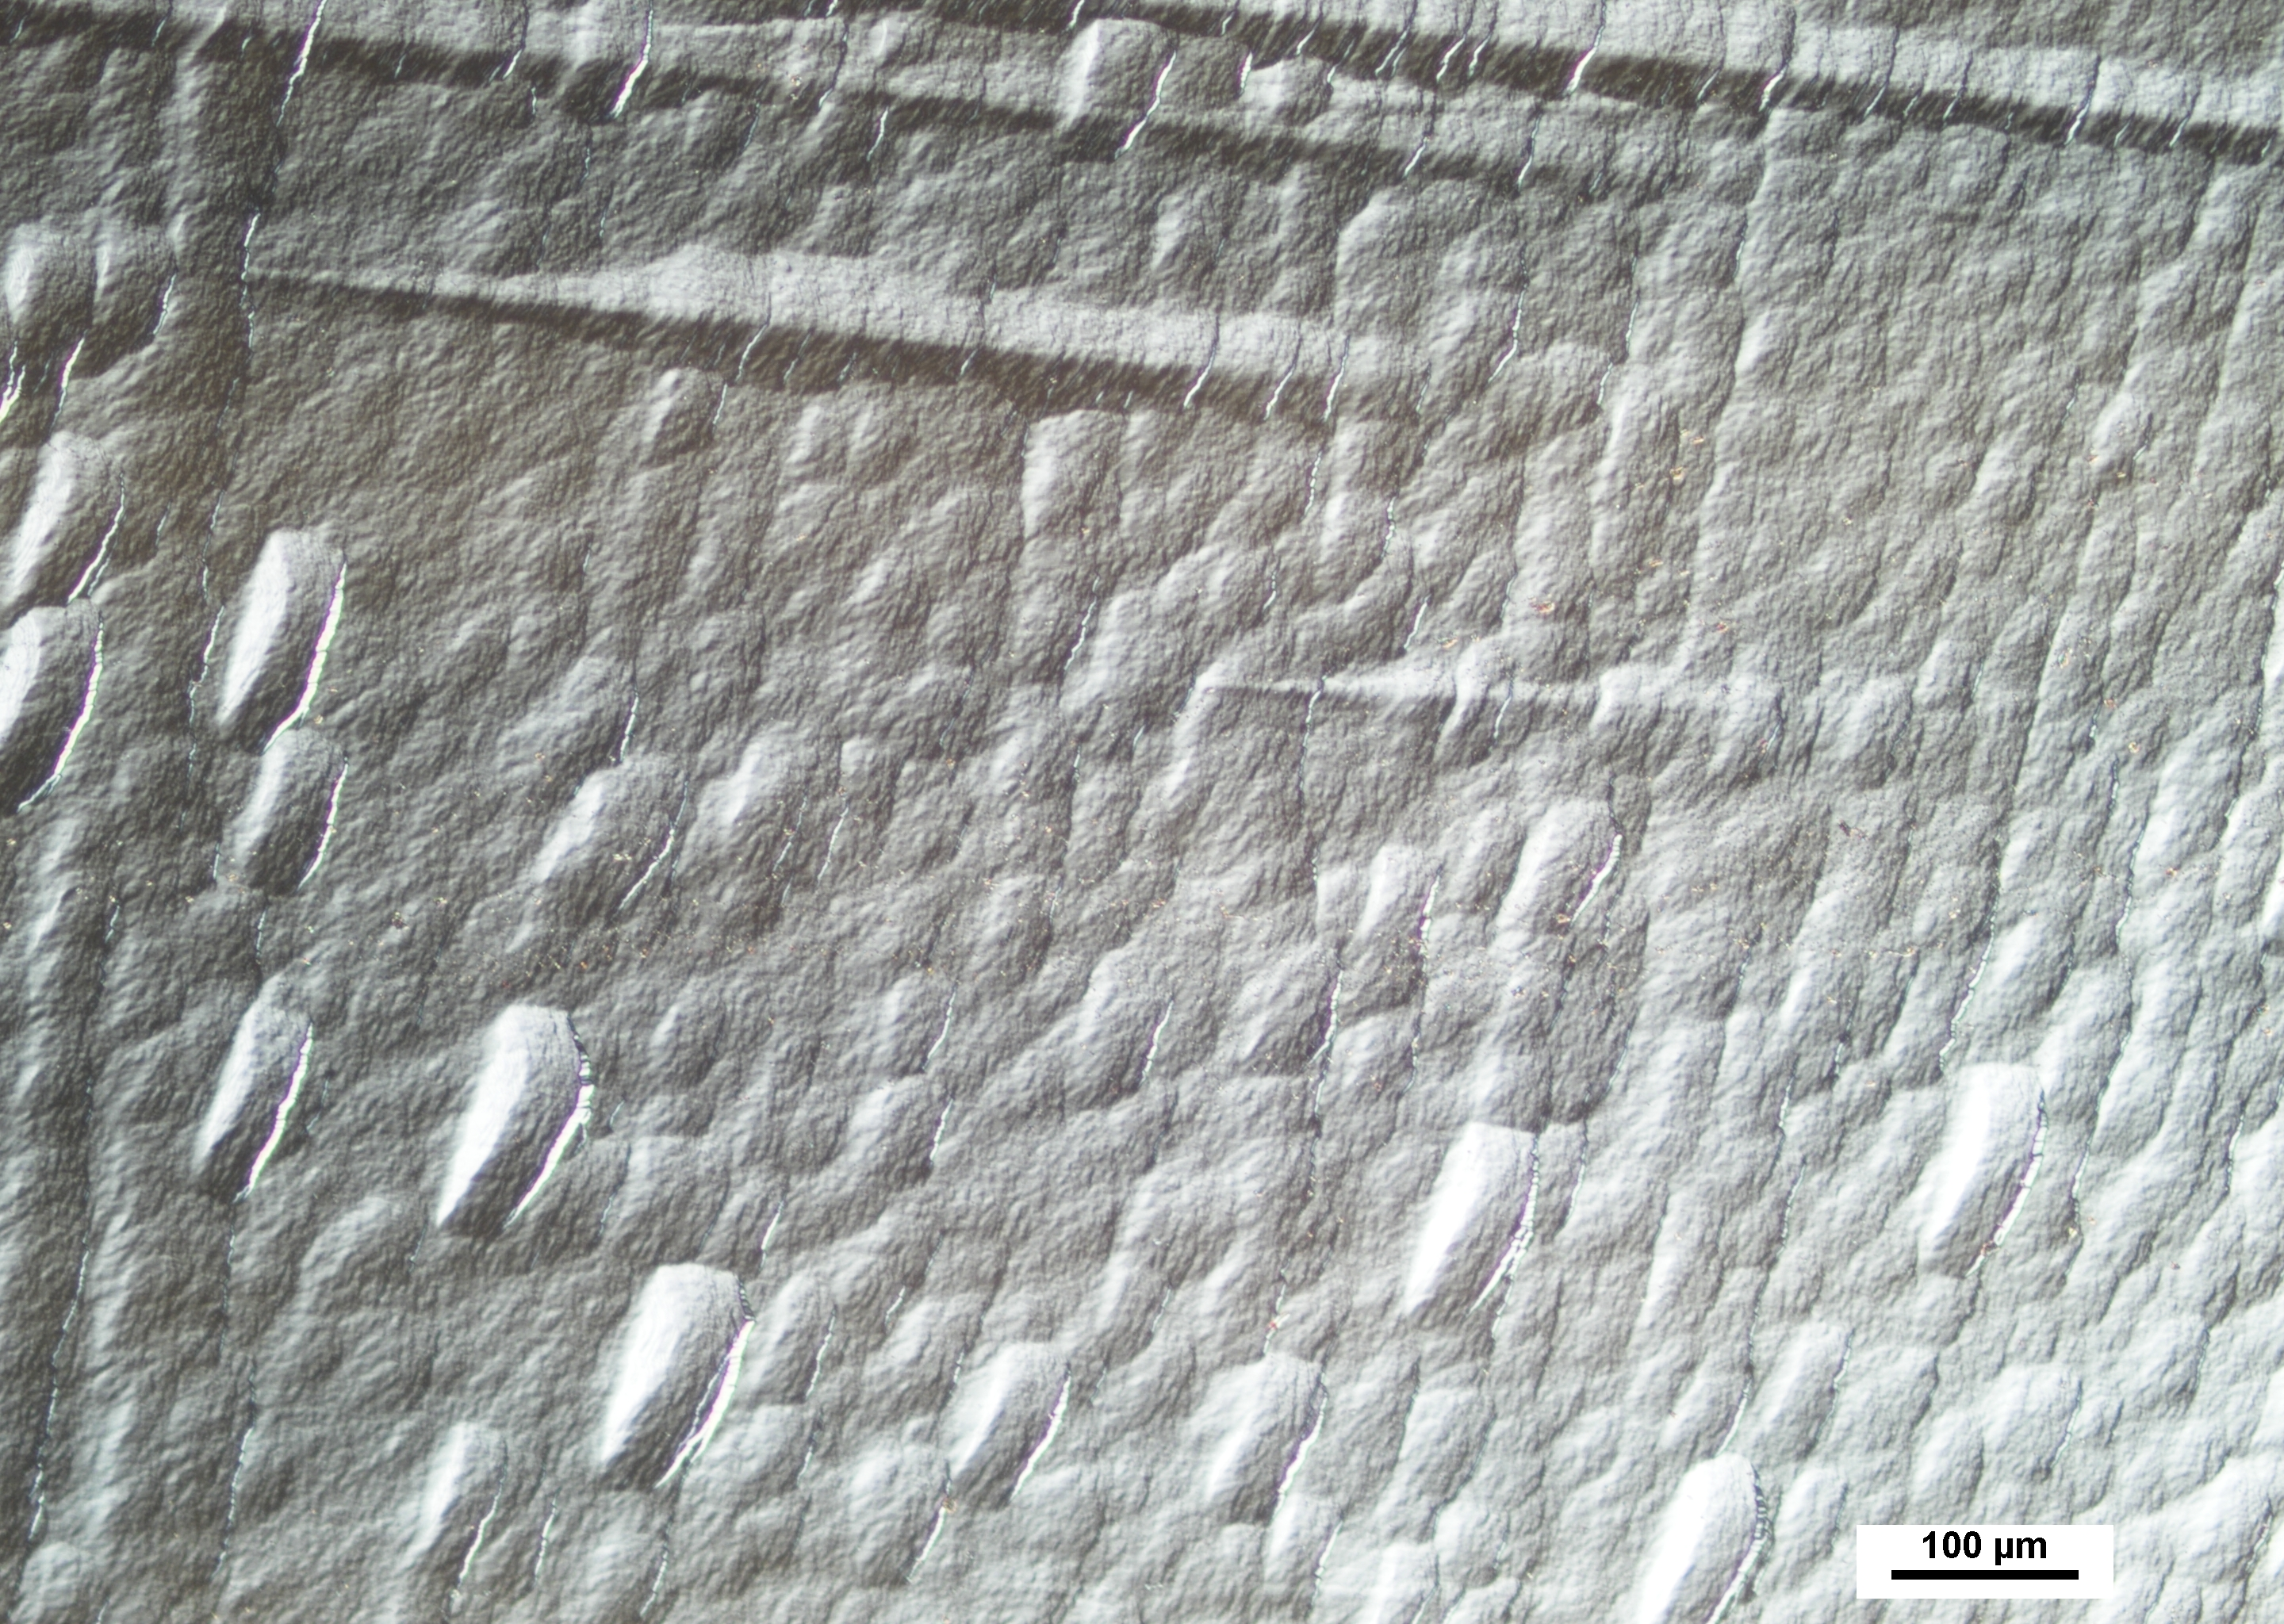
\includegraphics[scale = 0.05]{figures/SR21c1_Morph.jpg}
				\caption{(c) 1050 $^{\circ}$C}
			\end{subfigure}
		\caption{DICM images showing the morphological results of the three samples grown at the indicated temperatures. Smooth step flow growth is observed in the sample grown at 950 $^{\circ}$C shown in (a). (b) and (c) show scalloped, orange peel morphology for the samples grown at 1000 $^{\circ}$C and 1050 $^{\circ}$C}
		\label{fig: TempOptMorph}
	\end{figure}

	Differential Interference Contrast Microscopy (DICM) was used to evaluate the sample morphology. Two types of morphologies were observed. The first type of morphology observed is called “orange peel” morphology, named for the appearance. This morphology indicates poor-quality growth where several growth sites initiating at adatoms grow into one another to form the layer, which is not ideal because dislocation density increases. The ideal morphology is “step flow” morphology which develops from growth along a step edge and is indicative of a good quality growth with minimal defects. The DICM results for the three temperatures tested are shown in Figure \ref{fig: TempOptMorph}. The highest temperature gave the most significant orange peel morphology while the lowest temperature (950 $^{\circ}$C) exhibited the best step flow morphology. Based on these results, the substrate temperature for the next set of depositions was selected to be 950 $^{\circ}$C.


\section{Initial Pressure Series}
	After determining the optimized temperature of 950 $^{\circ}$C, eight 3 mm x 3 mm x 0.25 mm (100) CVD substrates (MTI) were pre-characterized and cleaned, as described above, in the as-received condition. These samples were used to for two separate studies. First, to determine the effects of pressure on four samples at approximately 1.5$^{\circ}$ offcuts (called pressure trials or initial pressure series). The second used three samples at lower offcuts to verify the previous results and one sample at a higher offcut than the initial series of approximately 2$^{\circ}$ offcut (called offcut series or offcut trials). Additional spectroscopic pre-characterization measurements were taken for these samples to determine the nitrogen incorporation. The total gas flow rate during deposition for these trials was reduced while keeping the ratios constant to fix the total flow rate at 400 sccm. Therefore, the flow rates were as follows: 368 sccm of H$_2$, 16 sccm of CH$_4$, and 16.5 sccm of 0.01 mol\% N$_2$ in H$_2$ giving total gas phase composition of 4\% carbon and 50 ppm of nitrogen. The 10-minute hydrogen etch was performed for each of these samples as well.
	
	The pressure series of depositions started with sample 21-20a. The 21-20a deposition pressure and temperature of 950 $^{\circ}$C and 290 mbar, respectively, were chosen to replicate the conditions found to be ideal in the previous temperature series. The pressure was increased for subsequent growths, i.e. 21-14a at 330 mbar followed by 21-15a at 370 mbar, and the final sample, 21-08a, was grown at the lowest pressure of 250 mbar to conclude the first pressure series trial. Orange peel growth was observed on 21-20a and 21-14a while 21-08a and 21-15a, which were grown at the extreme pressures of the study, showed good step flow growth. Unepitaxial crystallites were present on samples 21-14a and 21-15a, thus, leading to the conclusion that the ideal conditions for deposition, based on morphology alone, were 950 $^o$C and 250 mbar.
	\begin{FlushLeft}
		\begin{table} [h]
			\caption{Sample morphology vs (100) Offcut and Reactor pressure}
			\label{PressureMorphology}
			\begin{tabular}{|c|c|c|c|c|}
				\hline
				(100) Offcut  & 250 mbar  & 290 mbar & 330 mbar & 370 mbar \\
				($^{\circ}$) &  &  &  & \\
				\hline
				& 21-19a& 21-10a & & 21-11a\\
				$\approx$ 0.5 & {\includegraphics[scale =0.03]{figures/21_19a_Morph.jpg}} & {\includegraphics[scale =0.03]{figures/21_10a_Morph.jpg}}& X & {\includegraphics[scale =0.03]{figures/21_11a_Morph.jpg}} \\
				\hline
				& 21-08a & 21-20a & 21-14a & 21-15a\\
				$\approx$ 1.5 & {\includegraphics[scale =0.03]{figures/21_08a_Morph.jpg}} & {\includegraphics[scale =0.03]{figures/21_20a_Morph.jpg}} & {\includegraphics[scale =0.03]{figures/21_14a_Morph.jpg}} &  {\includegraphics[scale =0.03]{figures/21_15a_Morph.jpg}}\\
				\hline
				& 21-09a & & & \\
				$\approx$ 2.0 &{\includegraphics[scale =0.03]{figures/21_09a_Morph.jpg}} & X & X & X\\
				\hline
			\end{tabular}
		\end{table}
	\end{FlushLeft}
	\indent
	
	Later post characterization results (discussion to follow) lent itself to repeating some of the conditions (250 mbar, 290 mbar, and 370 mbar). The samples chosen for these repeats (21-19a, 21-10a, and 21-11a) were of a lower offcut than the initial samples. All three of these samples exhibited an orange peel morphology which seems to indicate that a lower offcut results in a poor growth morphology. To substantiate this, one final deposition was done at 950 $^{\circ}$C and 250 mbar on sample 21-09a, which was at a higher offcut of approximately 2$^{\circ}$ with respect to the (100) surface. Sample 21-09a exhibited orange peel morphology indicating that the offcut of the sample does not correlate with growth morphology. Morphological results are shown in Table \ref{PressureMorphology}.
	
	Several spectroscopic analysis techniques were used to characterize the defect incorporation in each sample. Fourier Transform Infrared (FTIR) spectroscopy had been used previously to determine boron concentration in boron doped diamond \cite{Demlow2014}. Therefore, FTIR spectra were taken before and after deposition to observe differences in the spectra after nitrogen doped growth on the pressure series. FTIR was not taken on samples for the temperature series as the HPHT substrate background nitrogen content would have dominated the results. As mentioned previously, the first sample growth for this series was 21-20a at the same conditions as the ideal conditions selected from the temperature series (950 $^{\circ}$ and 290 mbar), then pressure was increased incrementally for subsequent substrates and a low pressure concluded the series. Results are shown in Figure \ref{fig: FTIRInitial}.


 	Defined peaks at approximately 1330 cm$^{-1}$ and 2930 cm$^{-1}$ were visible on the first sample grown, 21-20a, and decreased in intensity for subsequent growths. This introduced the suspicion of contamination in the system, possibly due to the new sample holder or quartz dome. 
 	
 	A second series of growths, at the same conditions as the previous four but with lower offcuts, were completed to investigate the potential contamination. These results are shown in Figure \ref{fig: FTIRLowOffcut}
 
  	Not only did the 1330 cm$^{-1}$ and 2930 cm$^{-1}$ peaks persist, but the intensity of each peak was also greater than in the original series, suggesting a dependence on offcut. One additional sample was grown at 250 mbar and 950 $^{\circ}$C with an offcut of 2$^{\circ}$ with respect to the (100) surface, greater than the previous samples, to study the effects of offcut on the FTIR spectrum. These results are shown in Figure \ref{fig: FTIR250}. The results of this final deposition did not indicate a correlation between offcut and the intensity of the 1330 cm$^{-1}$ and 2930 cm$^{-1}$ peaks. 
 	
 	 \begin{figure} [H]
 		\begin{center}
 			\includegraphics[scale=0.75]{figures/FTIRInitalSeries.png}
 			\caption{FTIR spectra of the first four samples grown to evaluate temperature. Defined peaks are present at 1330 cm$^{-1}$ and 2930 cm$^{-1}$ for sample 21-20a.}
 			\label{fig: FTIRInitial}
 		\end{center}
 	\end{figure}
 	
 	\begin{figure} [H]
 		\begin{center}
 			\includegraphics[scale=0.75]{figures/FTIRLowOffcut.png}
 			\caption{FTIR spectra of the three samples grown to investigate potential contamination. Defined peaks at 1330 cm$^{-1}$ and 2930 cm$^{-1}$ persisted for samples 21-10a and 21-19a while diminishing for sample 21-11a, indicating these peaks are not due to contamination.}
 			\label{fig: FTIRLowOffcut}
 		\end{center}
 	\end{figure}
 	
 	 \begin{figure} [H]
 		\begin{center}
 			\includegraphics[scale=0.75]{figures/FTIR250mbar.png}
 			 
 			\caption{FTIR spectra of the final, higher offcut, sample compared to the two previous samples at the same conditions (950 $^{\circ}$C and 250 mbar). The lowest offcut sample, 21-19a at approximately 1$^{\circ}$ offcut to the (100) surface, exhibited the most defined 1330 cm$^{-1}$ and 2930 cm$^{-1}$ peaks. The sample with the lowest intensity of these peaks was the sample with an approximately 1.5$^{\circ}$ offcut, indicating no correlation.}
 			\label{fig: FTIR250}
 		\end{center}
 	\end{figure}
 	
 	Ultra-violet visible spectroscopy (UV-Vis) has been used to identify types of nitrogen defects in diamond \cite{Luo2021}. The samples possessing the 1330 cm$^{-1}$ and 2930 cm$^{-1}$ FTIR peaks were visibly dark, brown in color. UV-Vis spectroscopy was used to quantify this color and compare normalized absorption. Of the first four samples grown, 21-20a (290 mbar) appeared darkest in color, followed by 21-14a (330 mbar). The remaining two samples, 21-15a (370 mbar) and 21-08a (250 mbar), appeared nearly colorless. Figure \ref{fig: UVVisInitial} shows the UV-Vis spectra of these four samples. Sample 21-20a (290 mbar) exhibited the greatest absorption followed by 21-14a (330 mbar), consistent with naked-eye observations. The spectra of samples 21-15a (370 mbar) and 21-08a (250 mbar) appeared like those of pure diamond, with very little absorption in the UV-Vis region. 
 	
 	UV-Vis spectroscopy was also used to determine quantitative amounts of neutral substitutional nitrogen (N$_s^0$) \cite{Luo2022}. This was done via fitting three defect peaks (270nm, 360 nm, and 520 nm for N$_s^0$, vacancy clusters, and neutral nitrogen vacancy hydrogen defect (NVH$^0$) where the nitrogen, vacancy, and hydrogen are all replacing a carbon on a carbon lattice site, respectively), an electronic grade offset, and a ramp function in summation to fit to UV-Vis data. This method was attempted to determine the nitrogen concentration in the grown layers, however, the expected nitrogen concentration in the samples grown in this study (less than 5 ppm) was below the lower limit tested in the study by Luo \textit{et al.} and therefore did not prove useful for these approximations. 
 	
	\begin{figure}
		\begin{center}
			\includegraphics[scale=0.6]{figures/UVVisInitial.png} 
			\caption{UV-Vis spectra of the second series of growths, lower offcut, used to study the effects of pressure while eliminating the concern of potential contamination.}
			\label{fig: UVVisInitial}
		\end{center}
	\end{figure} 	 	

	The UV-Vis results of the second series of growths are shown in Figure \ref{fig: UVVisLowOffcut}. The greatest absorption is, again, observed at 290 mbar with sample 21-10a. Contrary to the previous results, the lower pressure (250 mbar) showed considerable absorption, more so than pure diamond, again suggesting a dependence on substrate offcut because this series was grown on substrates of a lower offcut than the first. 

	\begin{figure}[H]
		\begin{center}
			\includegraphics[scale=0.6]{figures/UVVisLowOffcut.png} 
			\caption{The figure above shows the UV-Vis spectra of the second series of growths, lower offcut, used to study the effects of pressure while eliminating the concern of potential contamination.}
			\label{fig: UVVisLowOffcut}
		\end{center}
	\end{figure}

	\begin{figure}[H]
		\begin{center}
			\includegraphics[scale=0.68]{figures/UVVis250.png} 
			\caption{The figure above shows the UV-Vis spectra of the three samples grown at 950$^o$C and 250 mbar of varying offcuts. No correlation was observed between UV-Vis absorption and substrate offcut.}
			\label{fig: UVVis250}
		\end{center}
	\end{figure}

	Again, to investigate the effects of offcut, one final sample was grown at the 250 mbar and 950 $^{\circ}$C condition but with a larger offcut to compare to the previous samples. These results are shown in Figure \ref{fig: UVVis250}. No correlation between offcut and UV-Vis absorption was observed. The greatest absorption occurred in the sample with the highest offcut, however the second greatest absorption occurred in the sample with the lowest offcut. 

	\begin{figure} [H]
		\begin{center}
			\includegraphics[scale=0.7]{figures/RamanAsRec.png} 
			\caption{The spectrum above shows the Raman spectrum of an unused (100) MTI substrate to compare to after deposition spectra of the studied samples}
			\label{fig: RamanAsRec}
		\end{center}
	\end{figure}

	The last spectroscopic analysis used to characterize the samples was Raman spectroscopy, which can be used to determine the quality of diamond, through the ratio of \textit{sp$^2$} to \textit{sp$^3$} carbon in a sample, quickly and non-destructively. The intensity of the 1350 cm$^{-1}$ and 1575 cm$^{-1}$ peaks are a result of the \textit{sp$^2$} carbon and can be compared to the intensity of the 1332 cm$^{-1}$ peak that is a result of the \textit{sp$^3$} carbon \cite{Zaitsev2001}. Raman spectra were not taken on each sample prior to deposition, however, a spectrum was taken on a substrate from the same supplier (MTI) to compare. These results are shown in Figure \ref{fig: RamanAsRec}. Raman spectra were taken on all seven samples used to study pressure, except 21-20a, after deposition. All seven samples exhibited a sharp peak at 1332 cm$^{-1}$, indicating the presence of diamond, as shown in Figure \ref{fig: RamanData}. 
	
	\begin{figure}
		\begin{FlushLeft}
			\begin{subfigure}{0.3\textwidth}
				\includegraphics[scale=0.41]{figures/Raman2119a.png}
			\end{subfigure}
			\hfill
			\begin{subfigure}{0.3\textwidth}
				\includegraphics[scale =0.41]{figures/Raman2110a.png}
			\end{subfigure}
			\hfill
			\begin{subfigure}{0.3\textwidth}
				\includegraphics[scale=0.41]{figures/Raman2111a.png}
			\end{subfigure}
			\hfill
			\begin{subfigure}{0.3\textwidth}
				\includegraphics[scale =0.41]{figures/Raman2108a.png}
			\end{subfigure}
			\hfill
			\begin{subfigure}{0.3\textwidth}
				\includegraphics[scale =0.41]{figures/Raman2114a.png}
			\end{subfigure}
			\hfill
			\begin{subfigure}{0.3\textwidth}
				\includegraphics[scale=0.41]{figures/Raman2115a.png}
			\end{subfigure}
			\hfill
			\centering
			\begin{subfigure}{0.3\textwidth}
				\includegraphics[scale =0.41]{figures/Raman2109a.png}
			\end{subfigure}
		\caption{Raman spectra of all samples from the pressure effects study, with the exception of 21-20a. A sharp 1332 cm$^{-1}$ diamond peak is observed on all samples. Additionally, a broad peak at approximately 1450 cm$^{-1}$ was present at varying intensities on each sample. }
		\label{fig: RamanData}
		\end{FlushLeft}
	\end{figure}
	
	Additionally, all seven exhibited a broad peak at approximately 1450 cm$^{-1}$ indicating the presence of graphitic clusters, not uniformly distributed graphite, which is \textit{sp$^2$} carbon \cite{Zaitsev2001}. The broad peak at 1450 cm$^{-1}$ was present in the unused sample as well as the samples with a nitrogen doped grown layer.

	The last characterizing technique used was Atomic Force Microscopy (AFM) to measure the substrate roughness prior to deposition. These results are shown in Table \ref{AFMPressure}. When comparing substrate roughness to the metrics discussed in previous sections, the substrates with the greatest surface roughness correlate to the samples with the greatest UV-Vis absorption and FTIR peak intensity. These results suggest substrate roughness has a significant impact on the deposition layer quality and defect incorporation.
	
	\begin{table} [H]
		\begin{center}
			\caption{Substrate roughness (R$_a$) measured via AFM.}
			\label{AFMPressure}
			\begin{tabular}{|c|c|c|c|c|}
				\hline
				(100) Offcut  & 250 mbar  & 290 mbar & 330 mbar & 370 mbar \\
				($^{o}$) &  &  &  & \\
				\hline
				& (21-19a) & (21-10a) & & (21-11a)\\
				$\approx$ 0.5 & 0.56 $\pm$ 0.1 nm & 1.13 $\pm$ 0.3 nm & X & 1.63 $\pm$ 0.5 nm\\
				\hline
				& (21-08a) & (21-20a) & (21-14a) & (21-15a)v\\
				$\approx$ 1.5 & 1.65 $\pm$ 1.0 nm & 1.09 $\pm$ 0.5 nm & 0.99 $\pm$ 0.5 nm &  1.88 $\pm$ 0.7 nm \\
				\hline
				& (21-09a) & & & \\
				$\approx$ 2.0 & 0.90 $\pm$ 0.5 nm & X & X & X\\
				\hline
			\end{tabular}
		\end{center}
	\end{table}

	The morphological and spectroscopic results of the series of samples intended to study the effects of pressure and offcut on the quality of growth and nitrogen incorporation are inconclusive, however, the sample with the best results was 21-08a.  No correlations between pressure nor offcut with morphology, growth rate, FTIR spectroscopy, UV-Vis spectroscopy, or Raman spectroscopy were observed. The current hypothesis is that a variable not considered in this study, such as sample preparation, is the dominant factor in the quality and defect incorporation. This variable needs to be identified and thoroughly studied to obtain meaning from the results presented here.  	
\subsection{Morphology}
\subsection{UVVis}
\subsection{FTIR}

\section{Low Offcut Series}
\subsection{Morphology}
\subsection{UVVis}
\subsection{FTIR}

\section{High Offcut Series}
\subsection{Morphology}
\subsection{UVVis}
\subsection{FTIR}

\section{Now with surface prep}
\subsection{Morphology}
\subsection{UVVis}
\subsection{FTIR}